\section{Results} \label{section:higgs_results}
Expected 95\% Confidence Level upper exclusion limits on the Higgs Boson production cross-section have been derived for the Greedy Categorization. Asymptotic approximation has been used for the actual computation, by following the procedure described in the previous section. For the final results, Rochester corrections have been used, however no significant differences were observed among the two possible sets of corrections. Triple Gaussian analytic form has been used for the modeling of the Standard Model Higgs Boson signal. For the background, the envelope of analytic functions was used and accounts for the potential bias among the forms across all of the categories.

Figure~\ref{fig:higgs_results_limitsvsmass} shows results for the 95\% CL upper limits on the signal strength as a function of the Higgs mass. 11 different mass hypotheses have been tested, in the range [120, 130] GeV with a step of 1 GeV, and interpolated in between. The observed upper limit on the signal strength does not exhibit significant deviations and is within $1\sigma$ from the expectation around the 125 GeV mass. Figure~\ref{fig:higgs_results_limitsBRvsmass} shows the 95\% CL upper limits on the Higgs Boson Branching Fraction, $\mathcal{B}(\Htomm)$, decaying via 2 muons. Standard Model Higgs Boson production cross-section is assumed.

Table~\ref{tab:higgs_results_limits} summarizes the results of the exclusion limits calculation.
\begin{table}[h!]
    \centering
    \caption{95\% CL Upper Limits on the Standard Model Higgs Boson Signal Strength.}
    \begin{tabular}{lcccccc}
\hlinewd{1.2pt}
\multirow{2}{*}{$m_\textup{h}$ [GeV]} & \multicolumn{5}{c}{Expected Limits} & \multirow{2}{*}{Observed limit} \\
\cline{2-6}
& $-2\sigma$ & $-1\sigma$ & median  & $1\sigma$ & $2\sigma$ & \\
\hline
120 & 1.08 & 1.44 & 2.02 & 2.84 & 3.84 & 1.90\\ 
121 & 1.07 & 1.44 & 2.01 & 2.83 & 3.82 & 1.50\\ 
122 & 1.07 & 1.43 & 1.99 & 2.83 & 3.82 & 1.63\\ 
123 & 1.07 & 1.43 & 1.99 & 2.83 & 3.85 & 2.28\\ 
124 & 1.07 & 1.43 & 2.01 & 2.84 & 3.87 & 2.92\\ 
125 & 1.08 & 1.44 & 2.02 & 2.87 & 3.91 & 2.77\\ 
126 & 1.10 & 1.47 & 2.05 & 2.91 & 3.97 & 2.37\\ 
127 & 1.12 & 1.49 & 2.09 & 2.98 & 4.04 & 2.13\\ 
128 & 1.15 & 1.52 & 2.13 & 3.03 & 4.09 & 2.06\\ 
129 & 1.17 & 1.56 & 2.18 & 3.09 & 4.18 & 1.94\\ 
130 & 1.20 & 1.60 & 2.23 & 3.16 & 4.27 & 1.82\\ 
\hlinewd{1.2pt}
\end{tabular}

    \label{tab:higgs_results_limits}
\end{table}

\begin{figure}[hbp]
    \centering
    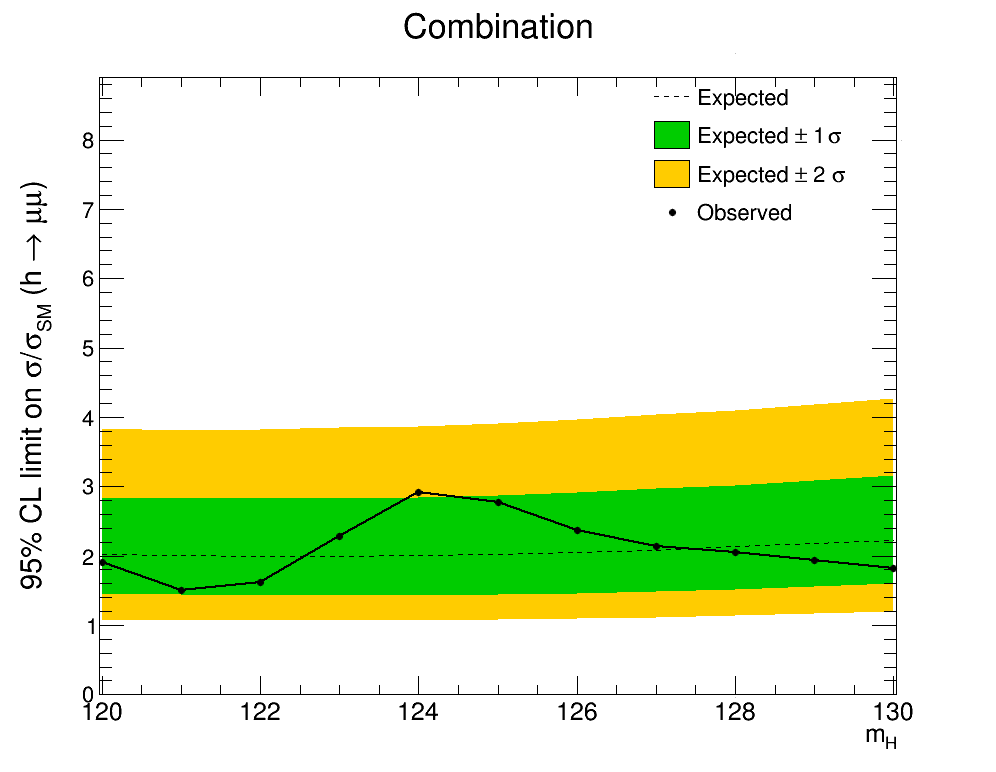
\includegraphics[width=0.9\textwidth]{figures/ch_higgs/limits/bdt_110to160_withSys_limits_1906/limitsByCategory__combTotal__TripleGaus.png}
    \caption{95\% CL Upper Limits on the Standard Model Higgs Boson Signal Strength as a function of mass. 11 mass hypotheses are tested and interpolated in between.}
    \label{fig:higgs_results_limitsvsmass}
\end{figure}
\begin{figure}[hbp]
    \centering
    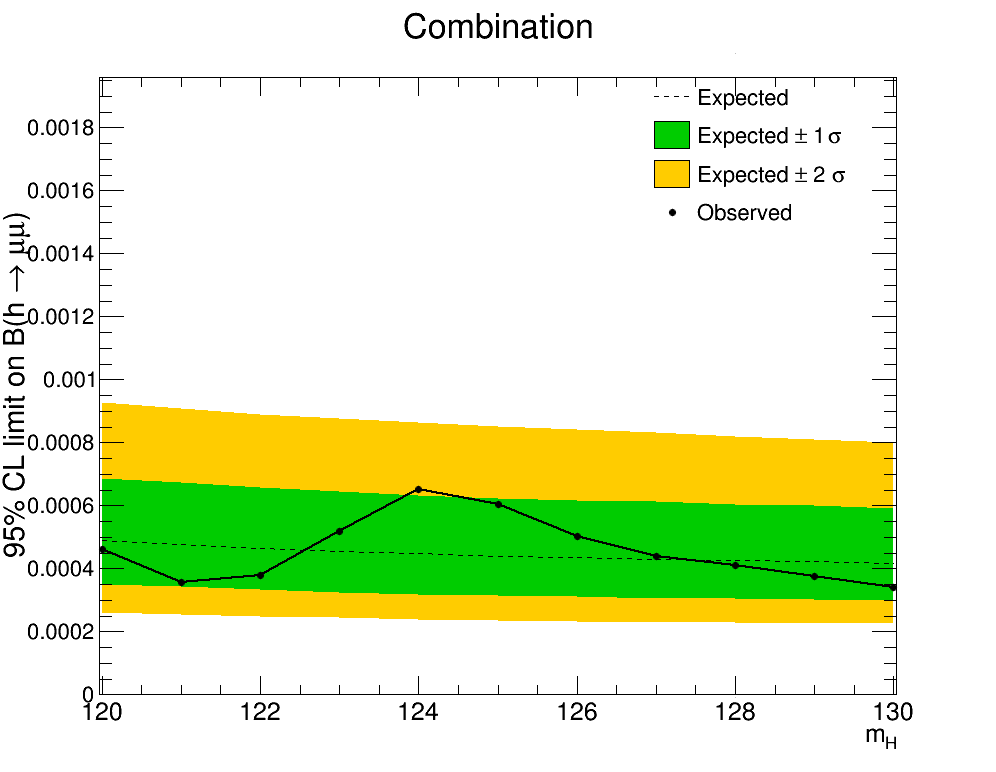
\includegraphics[width=0.9\textwidth]{figures/ch_higgs/limits/bdt_110to160_withSys_limits_1906/limitsOnBRByCategory__combTotal__TripleGaus.png}
    \caption{95\% CL Upper Limits on the $\mathcal{B}(\Htomm)$ as a function of mass Standard Model Higgs Boson production Cross-section is asssumed. 11 mass hypotheses are tested and interpolated in between.}
    \label{fig:higgs_results_limitsBRvsmass}
\end{figure}



% Expected 95\% CL upper limits on the signal strength modifier have been derived
% for the ``Bdt'' category based analysis and presented in
% Fig.~\ref{results:limit}. The expected limits are derived using the Asimov
% data-set ({\bf blind)}, using KF corrections and the following background
% functions:  BWZredux ( cat 0, 2, 3, 7, 8, 9, 10, 11, 12), Bernstein
% polynomial ( cat 1, 6), and SumExponential ( cat 4, 5). The expected
% significance at $\mH=125\,\gev$ for SM Higgs boson is $0.85~\sigma$.
% \begin{figure}[h!]
%     \centering
%     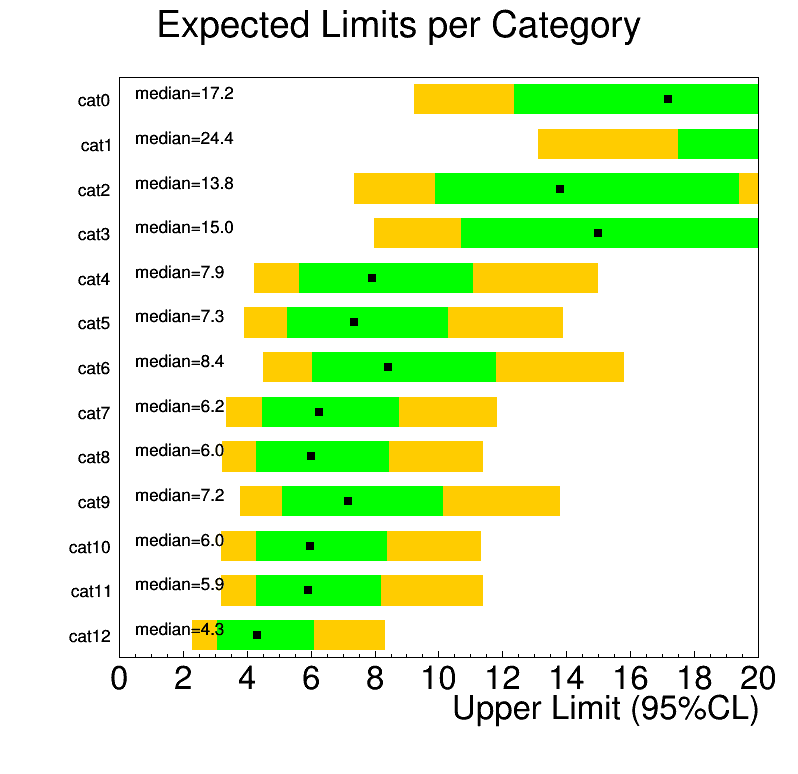
\includegraphics[width=0.681\textwidth]{figures/results/limitPerCategory}
%     \caption{The 95\% CL upper limit on the signal strength modifier. Each
% category is fitted independently. Limits are derived using the Asimov data-set
% ({\bf blind}). Systematic uncertainties are considered.}
%     \label{results:limit_splitted}
% \end{figure}




% Figure~\ref{results:mu} shows the best fit strength modifier,
% $\hat{\mu}=1^{+2}_{-1}$.
% \begin{figure}[h!]
%     \centering
%     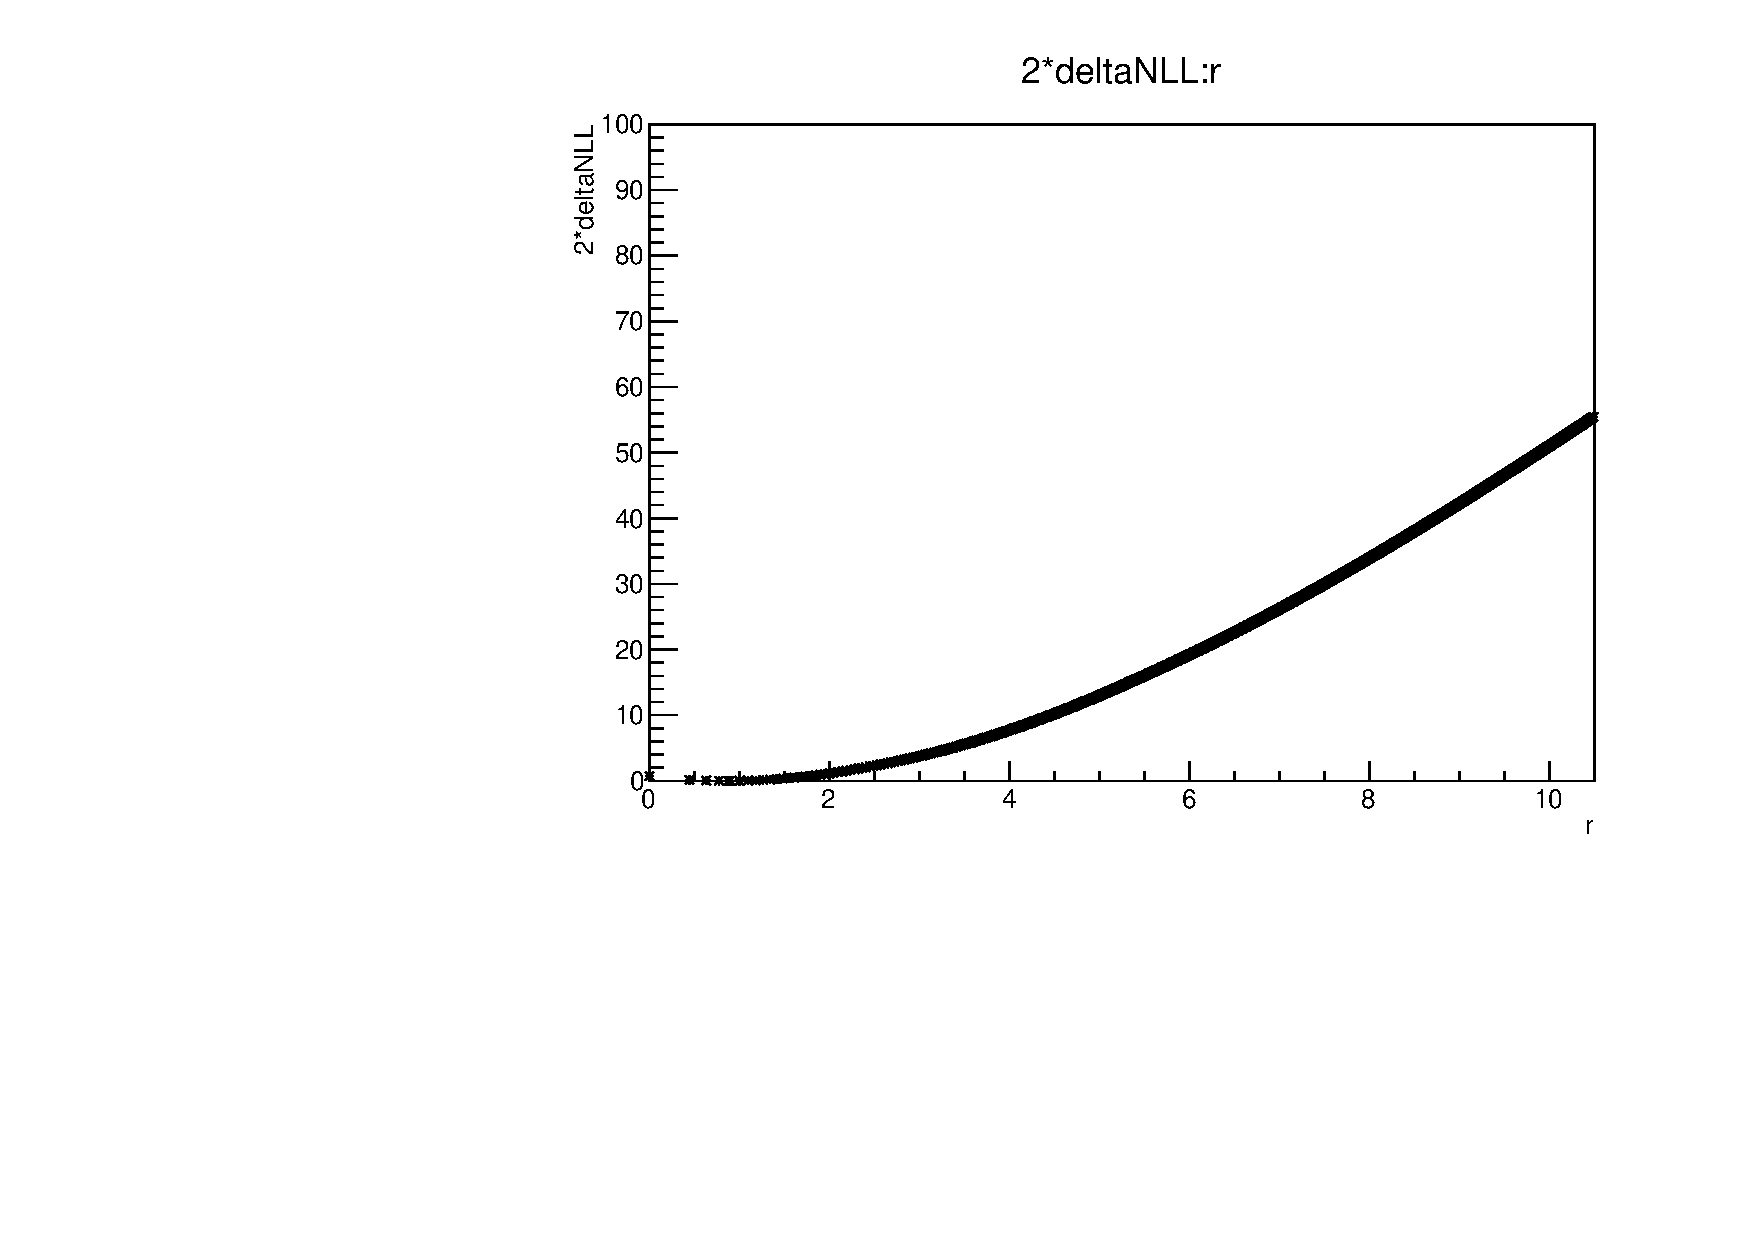
\includegraphics[width=0.681\textwidth]{figures/results/mu}
%     \caption{The $2\Delta\log{\mathcal{L}}$ versus $\mu$. Scans are derived using the Asimov data-set ({\bf blind}).}
%     \label{results:mu}
% \end{figure}

% Best fit of the strength modifier to the vector boson couplings (rV) and to
% the fermion couplings (rF), floated independently, can be seen
% in Fig.~\ref{results:rvrf}.
% \begin{figure}[h!]
%     \centering
%     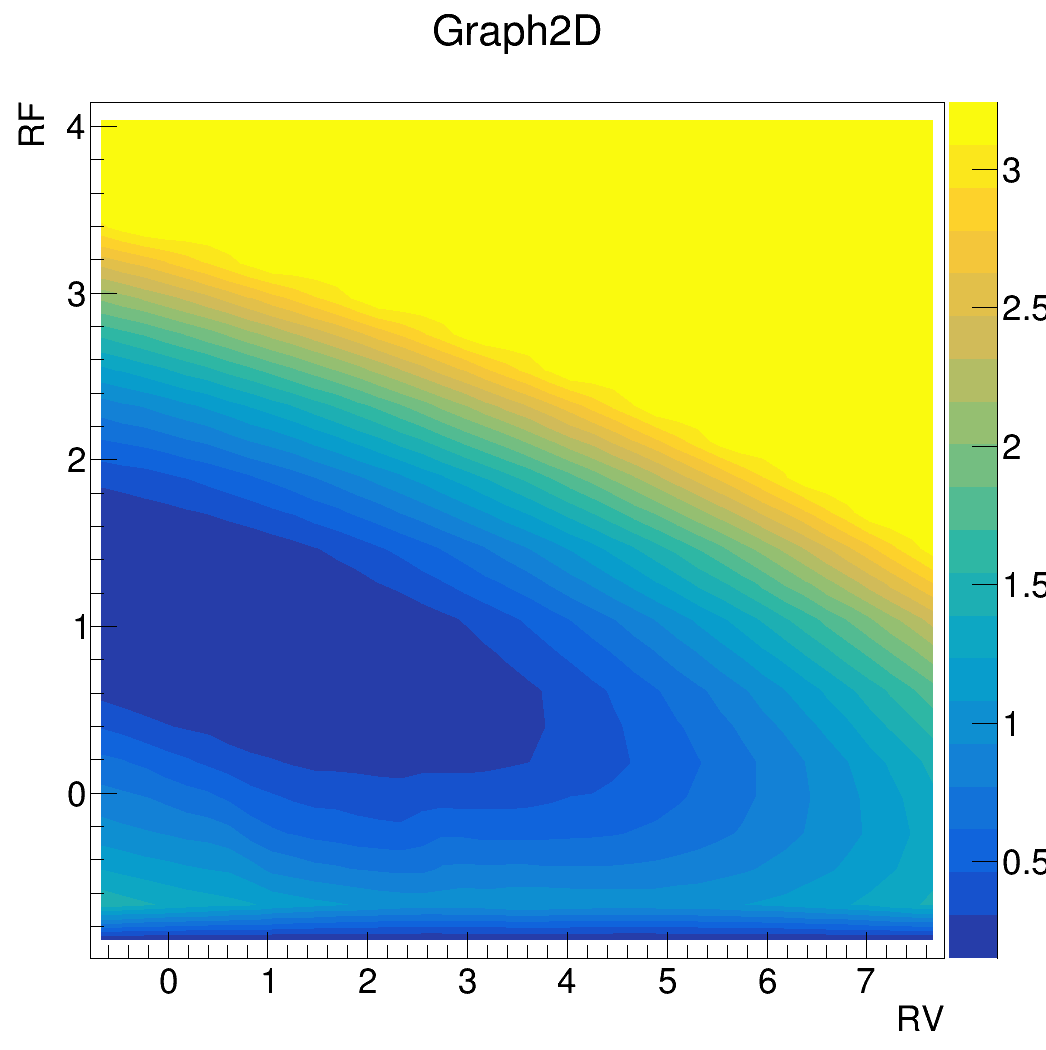
\includegraphics[width=0.681\textwidth]{figures/results/rV-rF}
%     \caption{The $2\Delta\log{\mathcal{L}}$ versus rV-rF. Scans are derived
% using the Asimov data-set ({\bf blind})}. Higgs boson mass is used as floating
% parameter.
%     \label{results:rvrf}
% \end{figure}


%\clearpage
%\subsection{Combination}
%Combined limits are performed using $7$ and $8\,\tev$ datacards as sumbitted to svn.
%Details of these analyses can be found in Ref. cite-RunI-FIXME %% ~\cite{RunI}

%The following changes are performed:
%\begin{itemize}
%\item The signal yields have been multiplied by the value of $\sigma(\text{proc},\mH)_{YR4}/\sigma(\text{proc},\mH)_{YR3}$
%\item The signal yields have been multiplied by the value of $\mathcal{B}(\Htomm)_{YR4}/\mathcal{B}(\Htomm)_{YR3}$
%\end{itemize}

%Nuisances are all uncorrelated (conservative).

%\begin{figure}[h!]
%    \centering
%    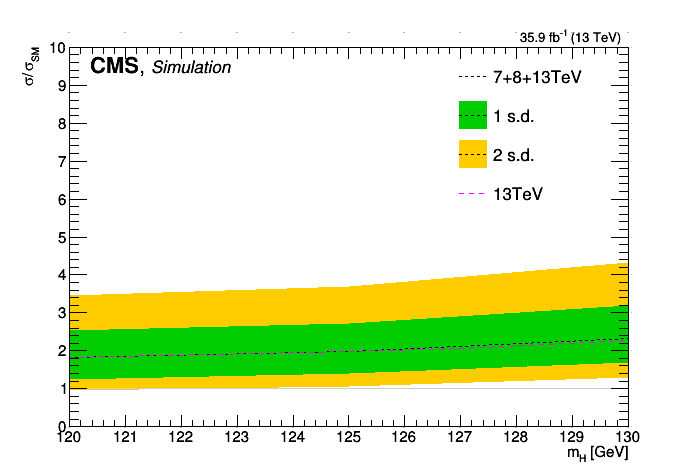
\includegraphics[width=0.681\textwidth]{figures/results/ExpLimitComb}
%    \caption{95\% CL upper limit on the signal strength modifier. Limits are derived using the Asimov dataset ({\bf blind})}
%    \label{results:comb_limit}
%\end{figure}

%\begin{table}[h!]
%    \centering
%    \caption{Combined Limits}
%    \begin{tabular}{lcccccc}
\hlinewd{1.2pt}
\multirow{2}{*}{$m_\textup{H}$ [GeV]} & \multicolumn{5}{c}{Expected Limits} & \multirow{2}{*}{Observed limit} \\
\cline{2-6}
& $-2\sigma$ & $-1\sigma$ & median  & $1\sigma$ & $2\sigma$ & \\
\hline
120 & 0.96 & 1.24 & 1.82 & 2.55 & 3.45 & - \\
125 & 1.05 & 1.41 & 1.98 & 2.73 & 3.69 & - \\
130 & 1.29 & 1.70 & 2.32 & 3.18 & 4.32 & - \\
\hlinewd{1.2pt}
\end{tabular}

%\end{table}
